\documentclass{article}
    % General document formatting
    \usepackage[margin=0.7in]{geometry}
    \usepackage[parfill]{parskip}
    \usepackage[utf8]{inputenc}
    \usepackage[T1]{fontenc}
    % Related to math
    \usepackage{amsmath,amssymb,amsfonts,amsthm, bm}
\usepackage{graphicx}

\begin{document}

\section {Budżet niepewności - Livox Mid 40}

Źródła niepewności: \\
\textbf{Przyrząd pomiarowy - Skaner laserowy Livox MID40 - Pomiar odległości}\\
Symbol : $r$\\
Metoda wyznaczenia : \textbf{B} (dane producenta)\\
Rozkład normalny \\
$\sigma_{r} = 2cm$

\textbf{Przyrząd pomiarowy - Skaner laserowy Livox MID40 - Pomiar kąta wiązki}\\
Symbol : $\theta, \phi$\\
Metoda wyznaczenia : \textbf{B} (dane producenta)\\
Rozkład prostokątny \\
$\sigma_{d} = \frac{0.1}{\sqrt{3}} \deg$


Pomiar położenia punktu w przestrzeni 3D jest wykonywany metodą pośrednią.
Skaner dokonuje pomiaru odległości i kąta odchylenia wiązki.
Funkcja pomiarowa $f(r,\theta, \phi)$ ma postać:
\begin{equation}
x = r \sin(\theta) \cos(\phi)
\end{equation}
\begin{equation}
y = r \sin(\theta) \sin(\phi)
\end{equation}
\begin{equation}
z = r \cos (\theta)
\end{equation}


\begin{equation}
F = \begin{bmatrix}
\frac{\partial f}{\partial r}&
\frac{\partial f}{\partial \theta}&
\frac{\partial f}{\partial \phi}=
\end{bmatrix}=
\left[\begin{matrix}\sin{\left(\phi \right)} \sin{\left(\theta \right)} & r \sin{\left(\theta \right)} \cos{\left(\phi \right)} & r \sin{\left(\phi \right)} \cos{\left(\theta \right)}\\\sin{\left(\theta \right)} \cos{\left(\phi \right)} & - r \sin{\left(\phi \right)} \sin{\left(\theta \right)} & r \cos{\left(\phi \right)} \cos{\left(\theta \right)}\\\cos{\left(\theta \right)} & 0 & - r \sin{\left(\theta \right)}\end{matrix}\right]
\end{equation}
\begin{figure}[htp!]
	\centering
	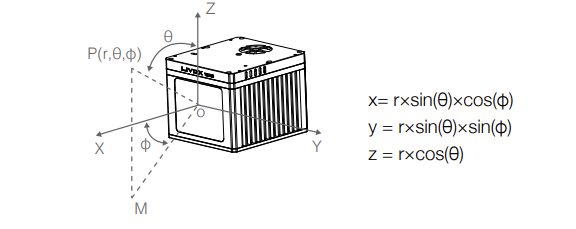
\includegraphics[width=0.7\linewidth]{livox_co.png}
	\caption{Układ wpółrzędnych}
	\label{fig:livoxco}
\end{figure}

Macierz kowariancji $\bm{\Sigma}$ jest dana:
\begin{equation}
\bm{\Sigma} =  \begin{bmatrix}
q_r^2 & 0 & 0 \\
0 & q_d^2 & 0 \\
0 & 0 & q_d^2 \\
\end{bmatrix}
\end{equation}




Macierz kowariaqncji pomiaru punktu 3D $\bm{\Sigma}_p$:
\begin{equation}
\bm{\Sigma}_p =  \bm{F} \bm{\Sigma} \bm{F}^\intercal
\end{equation}
Dla punktu obserwowanego na wprost lasera ($r=20m$, $\theta = 90 \deg$, $\phi = 0\deg$ ) w centymetrach kwadratowych:
\begin{equation}
\bm{\Sigma}_{pm} = 
\left[\begin{matrix}4.062 & 0 & 0\\0 & 4.0 & -3.77 \cdot 10^{-18}\\0 & -3.77 \cdot 10^{-18} & 4.062\end{matrix}\right]
\end{equation}

Dla punktu obserwowanego na skraju zakresu kątowego lasera ($r=20m$, $\theta = 110 \deg$, $\phi = 20 \deg$ ) w centymetrach kwadratowych:
\begin{equation}
\bm{\Sigma}_{ps} = 
\left[\begin{matrix}3.636 & 0.1352 & 0.006768\\0.1352 & 3.958 & 0.01859\\0.006768 & 0.01859 & 4.054\end{matrix}\right]
\end{equation}

Widoczna jest niewielka korelacja wspołrzędnej X wraz ze wspołrzędną Y mierzonego punktu. 
W celu wyznaczenia niepewności standardowej zostanie ona pominięta.
Niepewność rozszerzona pomiaru punktu oddalego o 20 metrów na wprost skanera laserowego Mid-40 wynosi:
\begin{equation}
\left[\begin{matrix}0 \\ 0 \\ 20000\end{matrix}\right] \pm \left[\begin{matrix} 6,02 cm \\ 6 cm \\ 6,02 cm\end{matrix}\right]
\end{equation}


\end{document}
